\chapter{Podstawy teoretyczne}
\section{Wyznaczanie położenia na podstawie odległości od punktów stałych}

Zadaniem prezentowanego prototypu jest wyznaczenie położenia nadajnika na podstawie
podległości od znanych punktów stałych. Niech $\boldsymbol{x}$ będzie szukanym punktem w przestrzeni,
$\boldsymbol{y_1,y_2,y_3}$ stałymi punktami o znanym położeniu, a $r_1,r_2,r_3$ wyznaczonymi odległościami, 
rysunek \ref{fig:polozenie}. 

\rysunekW{polozenie}{Wyznaczenie położenia na podstawie odległości od punktów stałych}{\label{fig:polozenie}}{0.7}
Wtedy $\boldsymbol{x}$ możemy wyznaczyć za pomocą układu równań:
\[
 \begin{cases}
    |\boldsymbol{y_1} - \boldsymbol{x}| = r_1
 \\ |\boldsymbol{y_2} - \boldsymbol{x}| = r_2
 \\ |\boldsymbol{y_3} - \boldsymbol{x}| = r_3
 \end{cases}
\]

co dla przestrzeni euklidesowej daje:
\[
 \begin{cases}
     (y_{11}-x_1)^2 + (y_{12}-x_2)^2 + (y_{13}-x_3)^2 = r_1^2
 \\  (y_{21}-x_1)^2 + (y_{22}-x_2)^2 + (y_{23}-x_3)^2 = r_2^2
 \\  (y_{31}-x_1)^2 + (y_{32}-x_2)^2 + (y_{33}-x_3)^2 = r_3^2
 \end{cases}
\]

Zauważmy, że znając odległość $\boldsymbol{x}$ od jednego punktu stałego wiemy, że $\boldsymbol{x}$ będzie leżał na
sferze o promieniu równym danej odległości. Znając dwie odległości możemy ograniczyć poszukiwania do części wspólnej dwóch sfer,
czyli okręgu. Dla znanych trzech odległości dostajemy część wspólną okręgu ze sferą, czyli dwa możliwe punkty.
Mimo, iż trzy odległości nie są wystarczające do jednoznacznego wyznaczenia $\boldsymbol{x}$, 
to otrzymane rozwiązania są na ogół od siebie daleko oddalone i bez większego problemu
możemy założyć, że jedno z rozwiązań jest naszym szukanym punktem.

Ponieważ mamy pełną dowolność w doborze punktów stałych $\boldsymbol{y_i}$ dla uproszenia możemy przyjąć:
$\boldsymbol{y_1}=(\frac{a}{2},0,0), \boldsymbol{y_2}=(-\frac{a}{2},0,0), \boldsymbol{y_3}=(0,h,0)$, czyli $\boldsymbol{y_1}, \boldsymbol{y_2}, \boldsymbol{y_3}$ są wierzchołkami
trójkąta równoramiennego o wysokości $h$ i podstawie $a$, wtedy układ równań upraszcza
się do postaci:
\[
 \begin{cases}
     (\frac{a}{2}-x_1)^2 + x_2^2 + x_3^2 = r_1^2
 \\  (\frac{a}{2}+x_1)^2 + x_2^2 + x_3^2 = r_2^2
 \\  x_1^2 + (h-x_2)^2 + x_3^2 = r_3^2
 \end{cases}
\]
z czego ostatecznie otrzymujemy:
\[
 \begin{cases}
     x_1 = \frac{r_2^2 - r_1^2}{2a}
 \\  x_2 = \frac{6r_2^2 - 4r_3^2 - 2r_1^2 + a^2}{8h}  + \frac{h}{2}
 \\  x_3 = \pm \sqrt{r_3^2-x_1^2-(h-x_2)^2}
 \end{cases}
\]


\section{Wyznaczanie orientacji w przestrzeni}


Kolejną rzeczą jaka nas interesuje jest orientacja w przestrzeni nadajnika.
Standardowo orientację zdefiniuje się jako kąty Eulera \cite{bib:katyEulera}: przechylenia, 
pochylenia oraz odchylenia wokół osi związanych z obiektem, jednak na nasze potrzeby wygodniej 
posługiwać się dwoma prostopadłymi wektorami, które jednoznacznie wyznaczają ów kąty. 
Prezentowany prototyp wyznacza położenie czterech punktów $\boldsymbol{x_1, x_2, x_3, x_4}$ znajdujących się
na nadajniku, a następnie na ich podstawie wyznacza poszukiwane dwa prostopadłe wektory które jednoznacznie
definiują jego orientację, rysunek \ref{fig:orientacja}.
 \begin{figure}[H]
    \centering
    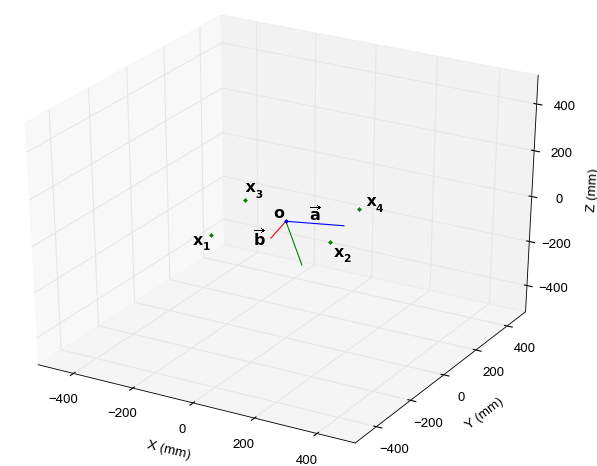
\includegraphics[width=0.5\textwidth, trim= 0mm 0mm 0mm 0mm,clip]{orientacja}
    \caption{Wyznaczanie orientacji na podstawie czterech punktów}
    \label{fig:orientacja}
\end{figure}
Na rysunku punkt $\boldsymbol{o} = (\boldsymbol{x_1} + \boldsymbol{x_2} + \boldsymbol{x_3} + \boldsymbol{x_4})/4$ jest szukanym położeniem
nadajnika, a wektory: $\boldsymbol{\overrightarrow{a}} = (\boldsymbol{x_2} + \boldsymbol{x_4})/2 - \boldsymbol{o}$ i 
$\boldsymbol{\overrightarrow{b}} = (\boldsymbol{x_1} + \boldsymbol{x_2})/2 - \boldsymbol{o}$ wyznaczają jednoznacznie
orientację przestrzenną nadajnika.

Zauważmy, że wyznaczenie położenia czterech punktów w przestrzeni daje nam pewną nadmiarowość
danych. Do wyznaczenia pozycji nadajnika potrzebujemy jedynie trzech współrzędnych,
a dla orientacji potrzebujemy jedynie trzech kątów, w sumie daje to sześć niewiadomych.
W prezentowanym podejściu wyznaczanych jest dwanaście niewiadomych co daje dwukrotną nadmiarowość danych.
Jest to efekt pożądany, ów nadmiarowość wykorzystywana jest do korekcji błędów pomiarowych.


\section{Pomiar odległości za pomocą ultradźwięków}

Prezentowane urządzenie do pomiaru odległości wykorzystuje metodę pomiaru czasu jaki 
potrzebuje dźwięk aby pokonać drogę od nadajnika do odbiornika,
rysunek \ref{fig:pomiar_odleglosci}.
\rysunekW{pomiar_odleglosci}{Pomiar odległości za pomocą ultradźwięków}{\label{fig:pomiar_odleglosci}}{0.4}

Znając prędkość rozchodzenia się fal dźwiękowych w powietrzy oraz czas jaki fala dźwiękowa potrzebowała
aby pokonać dany dystans jesteśmy w stanie wyznaczyć szukaną odległość.

Prędkość dźwięku w powietrzu jest mocno zależy od panujących warunków atmosferycznych \cite{bib:soundSpeed},  
głównym czynnikiem na nią wpływającym jest temperatura.
Dla gazu doskonałego prędkość wyraża się wzorem:
\[
V_{air} = 331,3  \frac{m}{s}  \sqrt{1+\frac{T}{273,15}}
\]
gdzie $T$ jest temperaturą w stopniach Celsjusza (\SI{}{\degC}).
Wzór ten możemy przybliżyć za pomocą rozwinięcia Taylora dla temperatur bliskich temperaturze pokojowej \SI{25}{\degC}:
\[
 V_{air} = (346,13  +  0,580(T - \SI{25}{\arcdeg})) \frac{m}{s}
\]

Mimo że współczynnik temperaturowy jest stosunkowo mały i stanowi jedynie \SI{0,17}{\%} całej prędkości
to przy pomiarach odległości rzędu metrów i rozdzielczościach rzędu milimetrów staje się on istotny, 
dlatego w prezentowanym prototypie istotną częścią stanowi kalibracja wstępna, podczas której
wyznaczana jest aktualna prędkość dźwięku.





